\documentclass[conference]{IEEEtran}
\usepackage{natbib}
\usepackage{graphicx}
\graphicspath{{./images/}}

\begin{document}
\title{Update for gazeNet\\
\thanks{Identify applicable funding agency here. If none, delete this.}
}

\author{\IEEEauthorblockN{1\textsuperscript{st} Lorenz Falcioni}
\IEEEauthorblockA{\textit{Fakultät Elektro- und Informationstechnik} \\
\textit{Ostbayerische Technische Hochschule Regensburg}\\
Regensburg, Germany \\
lorenzfalcioni@gmail.com}
\and
\IEEEauthorblockN{2\textsuperscript{nd} Timur Ezer}
\IEEEauthorblockA{\textit{Software Engineering Laboratory for Safe and Secure Systems (LaS³)} \\
\textit{Ostbayerische Technische Hochschule Regensburg}\\
Regensburg, Germany \\
timur.ezer@oth-regensburg.de}
\and
\IEEEauthorblockN{3\textsuperscript{rd} Jürgen Mottok}
\IEEEauthorblockA{\textit{Software Engineering Laboratory for Safe and Secure Systems (LaS³)} \\
\textit{Ostbayerische Technische Hochschule Regensburg}\\
Regensburg, Germany \\
juergen.mottok@oth-regensburg.de}
}

\maketitle
\section{Abstract}
gazeNet is a new framework for creating event detectors. The primary objective of this work is the update of the existing gazeNet by \citet{zemblys2018gazeNet} to current standards. In modifications this includes both in the used programming language i.e. Python2 to Python3 as well as the used packages. The existing code has also been modified to be interpretable on Windows-machines.

Furthermore an interface is provided to facilitate the application of the pretrained gazeNet. This is done by providiong a template for a script, which converts eye-tracking-data provided by the user in the appropriate format for gazeNet.


\section{Introduction}
The use of neural networks presents a new way of event detection in eye-tracking-data. \citet{zemblys2018gazeNet} presents gazeNet as one of the first approaches in the application of the technology. As much as the work of \citet*{zemblys2018gazeNet} represents a milestone in the evaluation of eye-tracking-data, since usability was not a priority, the use of gazeNet can be cumbersome, as it requires operation via a commandline and knowledge about the data structure being used.


\section{gazeNet}
The original gazeNet architecture by \citet{zemblys2018gazeNet} was inspired by Deep Speech 2 \citeauthor{deep_speech_2}, an end-to-end speech recognition neural network. gazeNet was implemented using the pyTorch6 neural network framework (version 0.2.0 4) and the starter code from Sean Naren.7 Our network has two onvolutional layers followed by three bidirectional recurrent layers with a fully connected layer on top. The convolutional layers use 2D filters with a size of 2 x 11 and are meant to extract deep features from raw input data, while the recurrent layers model event sequences and are responsible for detecting onsets and offsets of fixations, saccades and PSOs. \citet{zemblys2018gazeNet}

The presented framework gazeNet consists of various scripts written in python which allow the user to prepare raw data, augment data, train gazeNet and evaluate raw data.



\subsection{Update to gazeNet 1.1}
\subsection{Update to Python 3}

\subsection{Platform Independence}

\subsection{Validation of gazeNet 1.1}
\begin{figure}[h]
    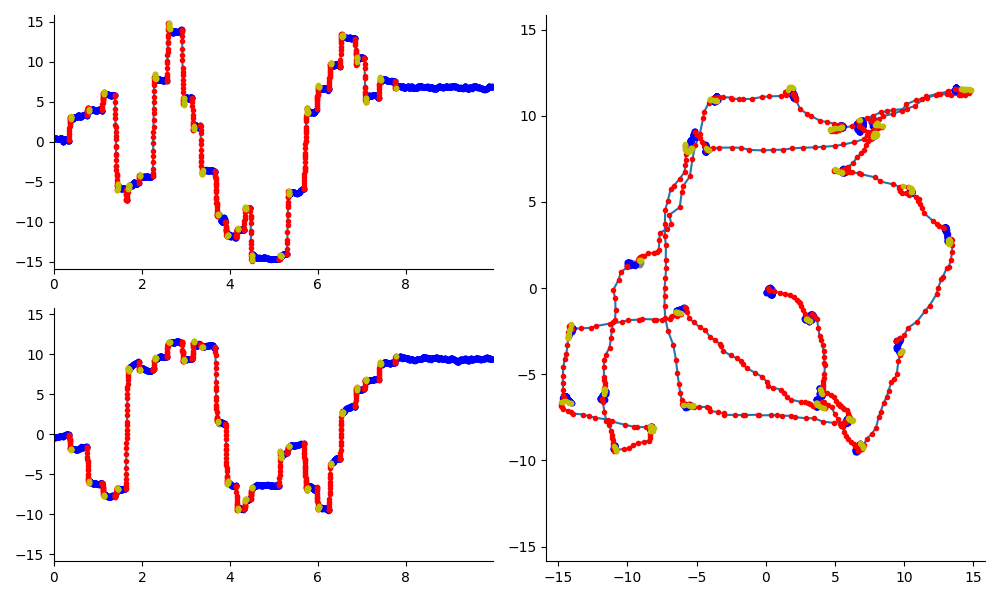
\includegraphics[width=\linewidth]{TH34_img_Europe_labelled_MN}
    \caption{The two graphs on the left show the x and y coordinates of the gaze position in degrees over time in seconds. The graph on the right resembles the gaze position in the x-y-plane. The red dots represent fixations, the blue dots represent saccades and the green dots represent post saccadic oscillations.}
\end{figure}

\section{Conversion script}
\begin{figure}[h]
    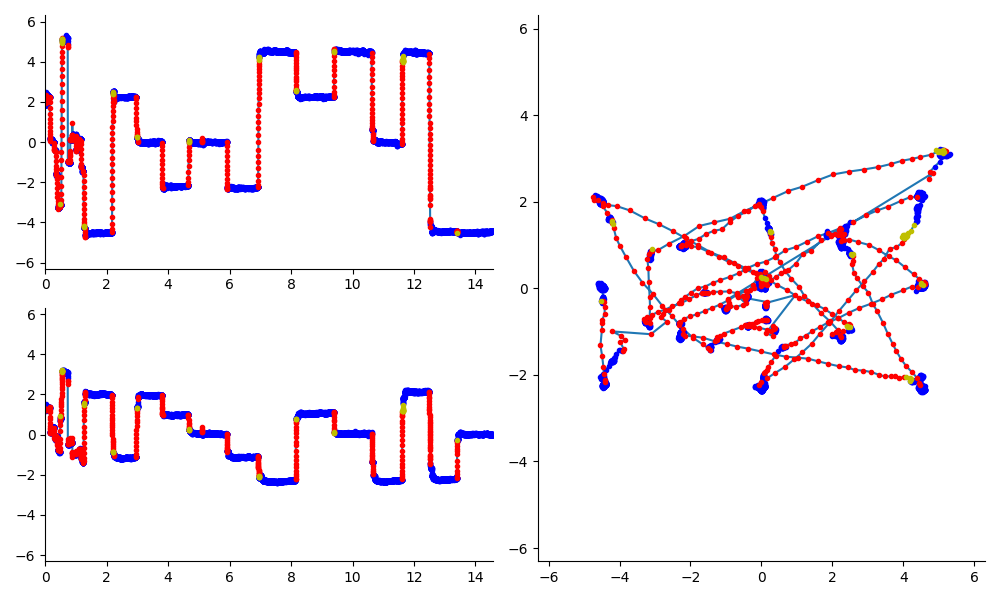
\includegraphics[width=\linewidth]{Kreuze_Random Recording1_short}
    \caption{The two graphs on the left show the x and y coordinates of the gaze position in degrees over time in seconds. The graph on the right resembles the gaze position in the x-y-plane. The red dots represent fixations, the blue dots represent saccades and the green dots represent post saccadic oscillations. It shoud be noted that the first two seconds of the recording contain the calibration points of the eye tracker. The calibration process contains events on which gazeNet is not trained. Therefore the labelling is insignificant.}
\end{figure}


\bibliographystyle{plainnat}
\bibliography{gazeNet.bib}
\end{document}